\chapter{Experimental Setup}\label{chap:setup}
This chapter provides a description of the hardware that makes up the experiment. Over the course of the project, the complexity of the experiment necessarily increased. The setup is presented in a bottom-up approach, starting from the most fundamental components, to provide a clear overview of the system. \\

\verysubsection{To-Do}
\begin{itemize}\item Figures describing each of the lasers
    \item Describe 3D and 2D MOT setups  
    \item Imaging systems
    \item Microwave synthesisers
    \item Raman Assembly
    \item MOT light distribution
\end{itemize}
\section{Chapter Overview}\label{sec:setup_overview}
The first two sections describe the two commercial laser systems used in this experiment. The \Muquans laser system which generates the light used for cooling and repump in the 2D and 3D \acp{mots}, referred to as the \acs{mot} light. The design and operation of this laser is given in \SectionRef{sec:setup_muquans}. A secondary laser system, built by MSquared, is used to generate light to drive Raman transitions between two hyperfine ground states in \ac{rb87}\footnote{The \Muquans laser also has a pair of lasers designed for driving Raman transitions, but these are not used in this experiment. \SectionRef{sec:setup_msquared} gives an explanation for this.}, otherwise referred to as Raman light. This is described in \SectionRef{sec:setup_msquared}.This is followed by a description of the vacuum chamber in \SectionRef{sec:setup_chamber} which contains both the 2D \ac{mot} (\SectionRef{subsec:setup_2DMOT}) and the 3D \ac{mot} (\SectionRef{subsec:setup_3DMOT}).  
\section{Vacuum Chamber}\label{sec:setup_chamber}
\subsection{The 2D MOT}\label{subsec:setup_2DMOT}
\subsection{The 3D MOT}\label{subsec:setup_3DMOT}
\subsection{Imaging Systems}\label{subsec:setup_imaging}
\subsubsection{CCD Camera}\label{subsubsec:setup_ccd}
\subsubsection{Photodiode}\label{subsubsec:setup_photodiode}

\section{The \Muquans Laser System}\label{sec:setup_muquans}
\verysubsection{To-Do}
\begin{itemize}
    \item Laser Schematic
    \item Plots of lock signals
    \item DDS Serial communication
    \item Power output, stability
    \item Refs for other experiments using Muquans systems
\end{itemize}
All the \ac{mot} light in this experiment was generated by the \Muquans laser \cite{muquansWebPage}. \Muquans is a French laser company that is a spin-off from the Institut d'Optique and Observatoire de Paris. Consequently, their technology has been developed over a long history of performing experiments into atom interferometry using Rubidium. A schematic of this laser system is shown in \FigureRef{fig:muquans_schematic}. The \Muquans laser is comprised of four 1560nm \acp{ECDLs} which are frequency-doubled to produce light at wavelengths close to 780nm. The telecommunications industry, which relies heavily on light in the 1530-1565nm wavelength band for optical communications, has motivated a rapid development in low-noise, robust lasers which are much more stable outside of laboratory conditions than their 780nm counterparts. The requirement for long-term stability of a laser system is one which many applications of quantum mechanics to technology will greatly benefit from by removing a need for frequent maintainence.

\begin{figure}
    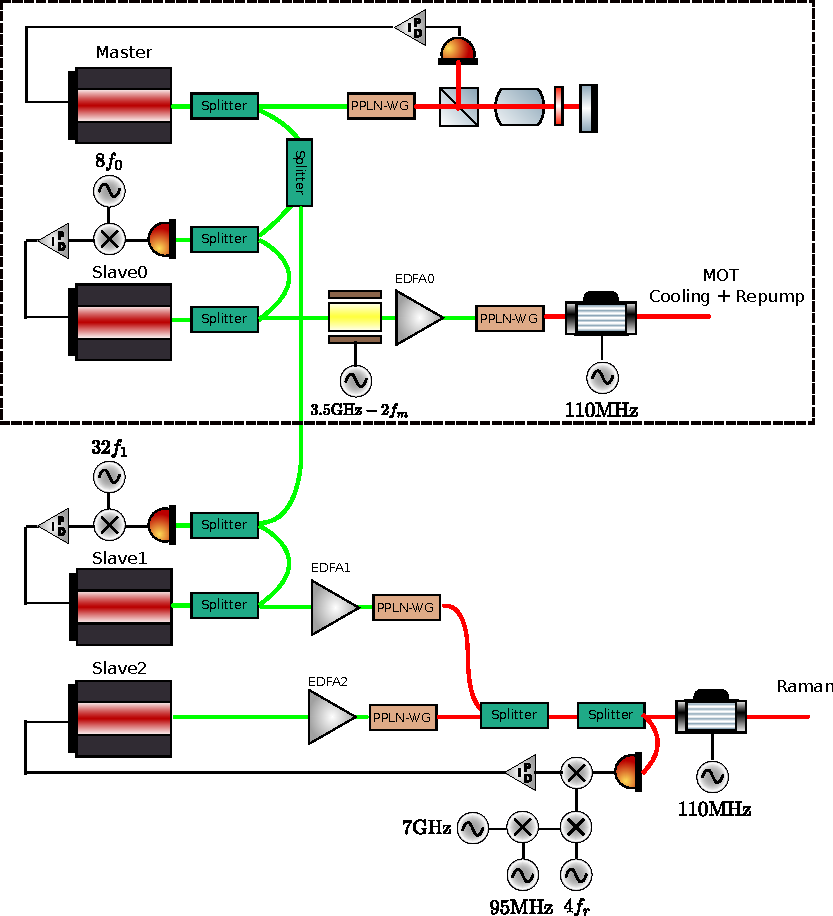
\includegraphics{muquans_schematic}
    \caption[\Muquans Laser System Diagram]{Schematic of the \Muquans laser system. Each output laser is derived from a 1560nm \acs{ecdl} (shown in green) which is amplified using an \acs{edfa} and then frequency-doubled to 780nm using a \acs{ppln} crystal. A master laser is locked to the 3,4 crossover in \ac{rb85} and the output lasers are offset-locked to their corresponding frequencies. The dashed region indicates the components used for generating light for the \acp{mots}, which was the only function of this laser for this experiment.}\label{fig:muquans_schematic}
\end{figure}
\subsection{Absolute Frequency Reference}
The purpose of the master laser is to provide an absolute frequency reference so that the MOT light and Raman light can be controlled by comparing the frequency difference of the slave lasers to this. The master laser is locked to the 3,4 crossover in \ac{rb85}, so that the 
\subsection{Generating MOT light}
\subsection{Raman light}
\subsection{Real-time Frequency Control}
\section{The M-Squared Laser System}\label{sec:setup_msquared}
\verysubsection{To-Do}
\begin{itemize}
    \item Schematic
    \item Raman PLL phase-noise
    \item Laser Control
    \item DCS module
\end{itemize}
\subsection{Raman Light}
\section{Raman Optical System}\label{sec:setup_ramanoptics}
\subsection{Vacuum design}\label{subsec:setup_ramandesign}
\subsection{Raman Beam Collimator}\label{subsec:setup_ramancollimator}
\subsection{Retro-reflection Assembly}\label{subsec:setup_ramanmirror}
\section{MOT Light Distribution}\label{sec:setup_lightdist}
\subsection{Optical Fibre Network}\label{subsec:setup_fibrenet}
\subsection{Power Control}\label{subsec:setup_lightpower}

\section{Microwave Field Generation}\label{sec:setup_microwave}
\subsection{Setup}\label{subsec:setup_microwave_setup}
\subsection{Wind-Freak Microwave Synthesiser}\label{subsec:setup_windfreak}arg